%%%%%%%%%%%%%%%%%%%%%%%%%%%%%%%%%%%%%%%%%
% Supplementary materials --- Paper 1
% Companion to skeleton.tex (ICES JMS / Fish and Fisheries draft).
% Four Celtic/Irish Sea gadoids only (no haddock, no mackerel).
% Stock order follows the main text: Celtic Sea cod, Irish Sea whiting,
% Irish Sea cod, Celtic Sea whiting.
% Figures regenerated by scripts/si_flstock_refpts.R and
% scripts/si_backtest_scenarios.R.
%%%%%%%%%%%%%%%%%%%%%%%%%%%%%%%%%%%%%%%%%
%!TEX program = xelatex
\documentclass[11pt,a4paper]{article}

\usepackage[margin=2.5cm]{geometry}
\usepackage{amsmath,amssymb}
\usepackage{booktabs}
\usepackage{graphicx}
\usepackage{setspace}
\usepackage{natbib}
\usepackage{hyperref}
\onehalfspacing
\setlength{\parindent}{0pt}
\setlength{\parskip}{0.5em}

\newcommand{\Fmsy}{F_{\mathrm{MSY}}}
\newcommand{\Blim}{B_{\lim}}
\newcommand{\Btrig}{\mathrm{MSY}_{B_{\mathrm{trigger}}}}
\newcommand{\Bmsy}{B_{\mathrm{MSY}}}
\newcommand{\Ftar}{F_{\mathrm{target}}}

\title{Supplementary materials\\[0.4em]
\large Supplement to ``Separating advice-rule performance from
implementation and productivity: a historical closed-loop backtest''}
\author{}
\date{}

\begin{document}
\maketitle

\noindent\textit{Companion to the main manuscript.} This supplement
documents the WGCSE assessment time series used to condition the
operating models (OMs) for the four demonstration stocks, with published
ICES reference points from the Stock Assessment Graphs database (SAG)
overlaid, and the Historical, open-loop $\Fmsy$ (benchmark), and Advice
rule trajectories. Throughout,
$\Ftar$ is the HCR target (published ICES $F_{\mathrm{MSY}}$ used as the
advice-rule control point); $\Fmsy$ and $\Bmsy$ denote OM MSY reference
points when used.

%==============================================================================
\section{Demonstration stocks and ICES reference points}
\label{sec:si-stocks}
%==============================================================================

The four demonstration stocks are Celtic Sea cod (\texttt{cod.27.7e-k}),
Irish Sea whiting (\texttt{whg.27.7a}), Irish Sea cod (\texttt{cod.27.7a}),
and Celtic Sea whiting (\texttt{whg.27.7b-ce-k}). Horizontal lines use the
same published ICES $\Blim$, $\Btrig$, and $\Ftar$ values as the SAG
screening table in the main text.
% Assessment objects: data/WGCSE/, listed in data/reference/stocks.csv.

\begin{table}[htbp]
\centering
\caption{Latest SAG terminal-year status and ICES reference points for the
four demonstration stocks (ratios as in the main-text status table;
absolute SSB, $F$, and reference points shown here). Values are from the
latest SAG assessment (column ``Ass.''), which can be a later vintage
than the WGCSE assessment used to condition the OM.}
\label{tab:si-casestudy-status}
\resizebox{\textwidth}{!}{%
\begin{tabular}{@{}lrrrrrrrrrr@{}}
\toprule
Stock & Ass. & Year &
  SSB/$\Btrig$ & SSB/$\Blim$ & $F/\Ftar$ &
  SSB & $F$ & $\Ftar$ & $\Blim$ & $\Btrig$ \\
\midrule
Celtic Sea cod     & 2026 & 2025 & 0.02 & 0.02 & 4.95 & 99    & 1.435 & 0.290 & 4200  & 5800 \\
Irish Sea whiting  & 2025 & 2024 & 0.53 & 0.73 & 4.14 & 1223  & 0.870 & 0.210 & 1670  & 2322 \\
Irish Sea cod      & 2026 & 2026 & 0.28 & 0.38 & 0.05 & 3584  & 0.009 & 0.171 & 9364  & 13012 \\
Celtic Sea whiting & 2026 & 2025 & 0.26 & 0.36 & 0.65 & 13014 & 0.242 & 0.375 & 36571 & 50818 \\
\bottomrule
\end{tabular}%
}
\end{table}

%==============================================================================
\section{Assessment time series with ICES reference points}
\label{sec:si-flstock}
%==============================================================================

Each figure is a four-panel assessment-style time series from the local
WGCSE assessment: recruitment (age~1 numbers), spawning biomass (SB),
catch, and mean fishing mortality ($\bar F$). On the SB panel, dashed
$\Blim$ and dotted $\Btrig$ are shown; on the $F$ panel, dashed $\Ftar$.
Values match Table~\ref{tab:si-casestudy-status}.

\begin{figure}[htbp]
\centering
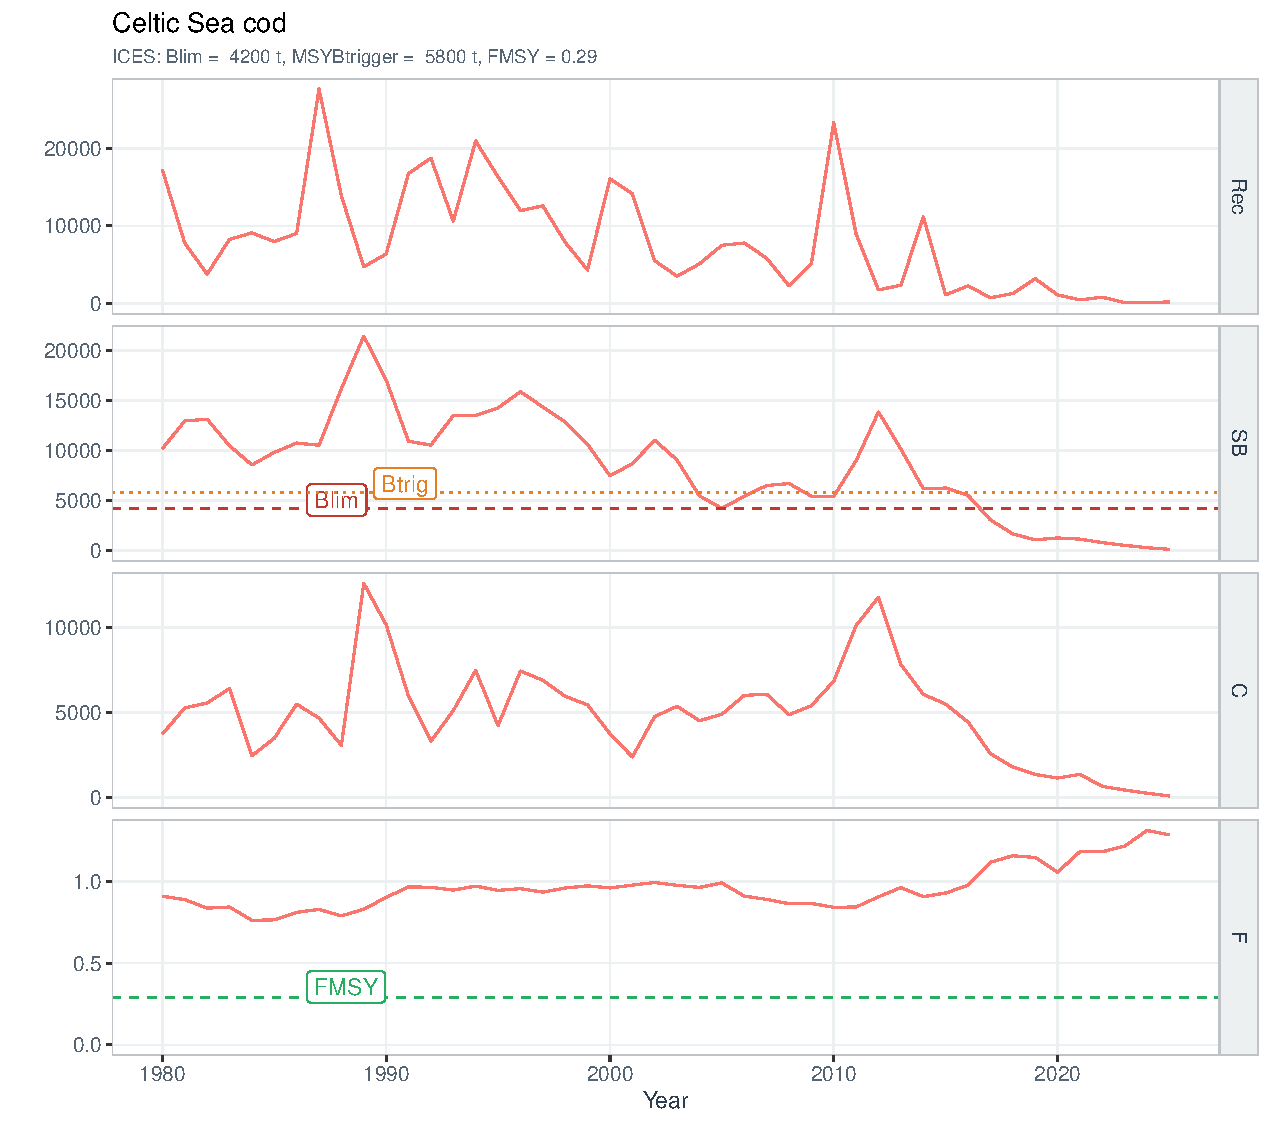
\includegraphics[width=\textwidth]{figs/si/si_flstock_cod.27.7e-k.pdf}
\caption{Celtic Sea cod (\texttt{cod.27.7e-k}). WGCSE assessment
recruitment, SSB, catch, and $\bar F$, with ICES $\Blim=4200$\,t,
$\Btrig=5800$\,t, and $\Ftar=0.290$.}
\label{fig:si-cod7ek}
\end{figure}

\begin{figure}[htbp]
\centering
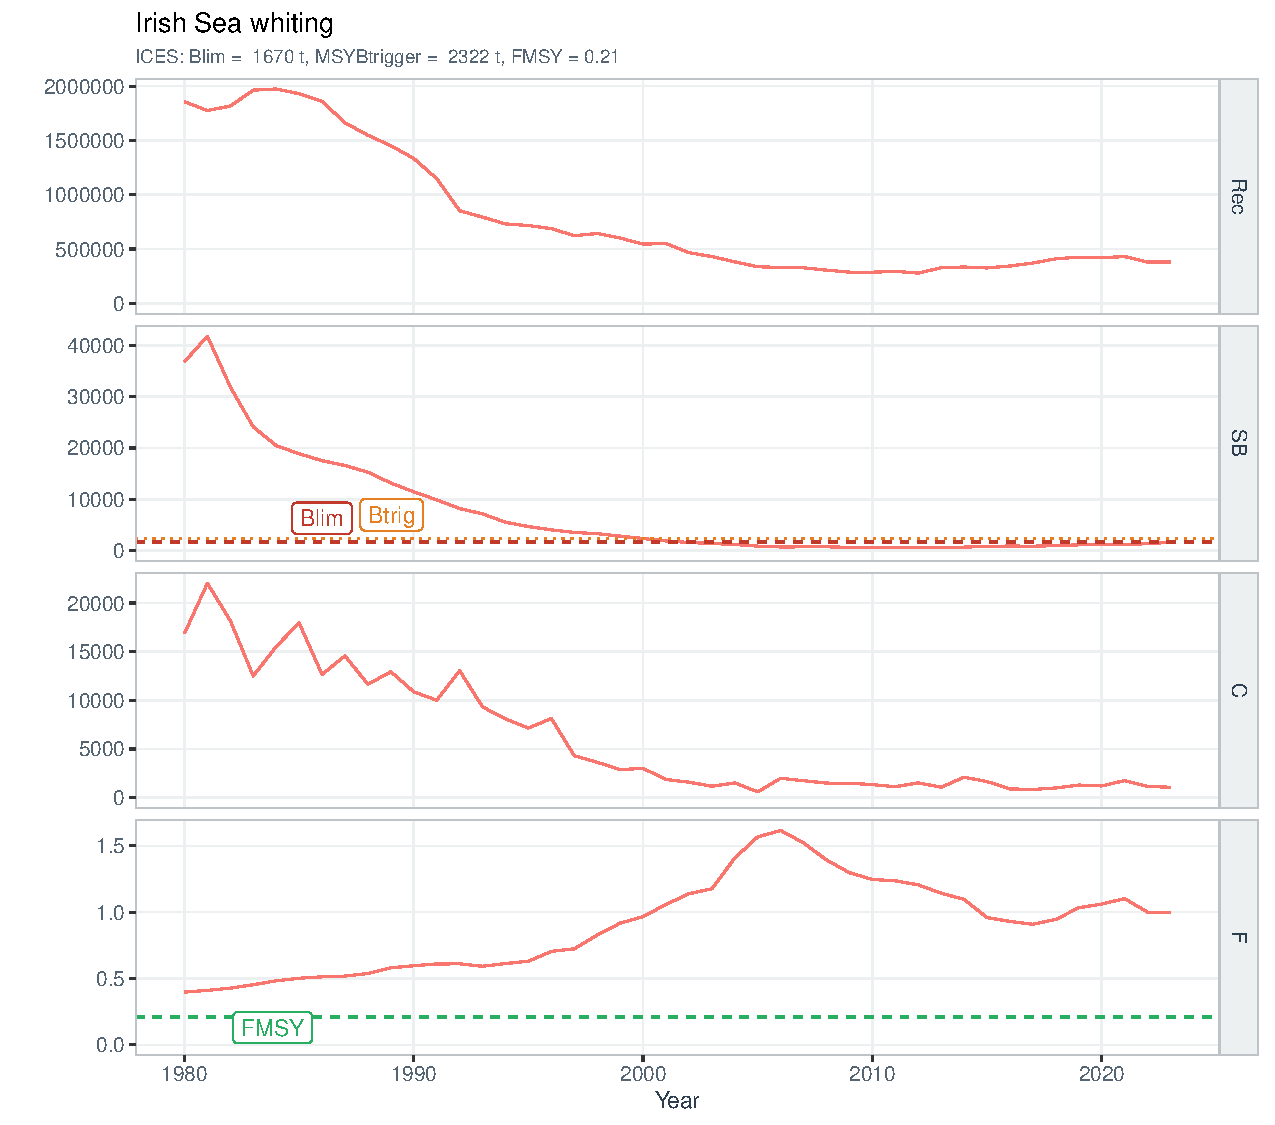
\includegraphics[width=\textwidth]{figs/si/si_flstock_whg.27.7a.pdf}
\caption{Irish Sea whiting (\texttt{whg.27.7a}). WGCSE assessment
recruitment, SSB, catch, and $\bar F$, with ICES $\Blim=1670$\,t,
$\Btrig=2322$\,t, and $\Ftar=0.210$.}
\label{fig:si-whg7a}
\end{figure}

\begin{figure}[htbp]
\centering
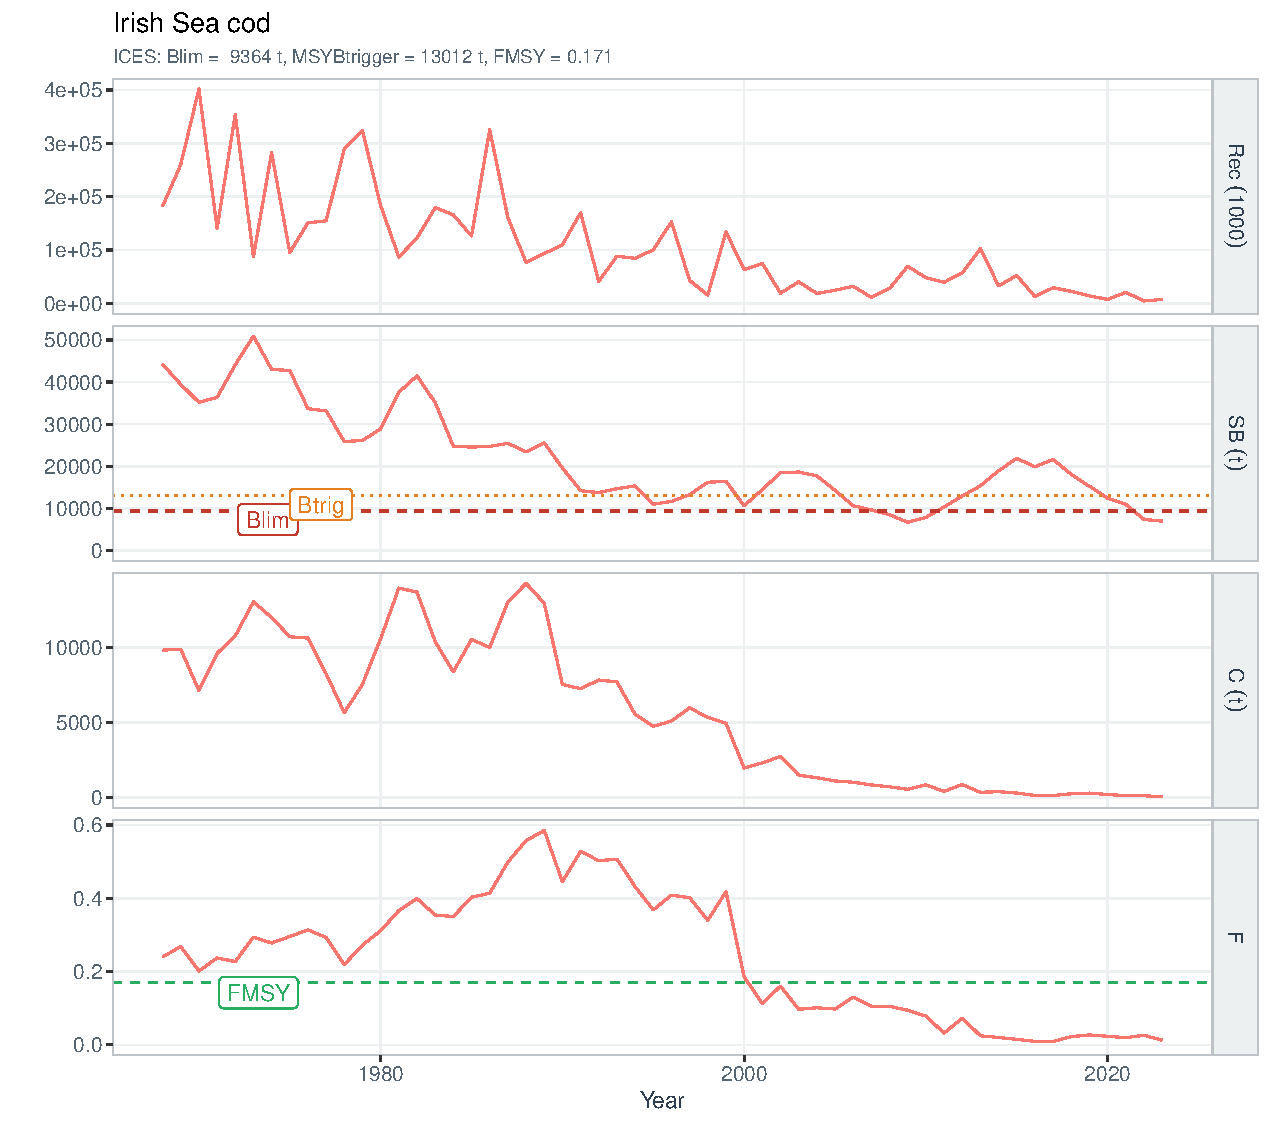
\includegraphics[width=\textwidth]{figs/si/si_flstock_cod.27.7a.pdf}
\caption{Irish Sea cod (\texttt{cod.27.7a}). WGCSE assessment
recruitment, SSB, catch, and $\bar F$, with ICES $\Blim=9364$\,t,
$\Btrig=13012$\,t, and $\Ftar=0.171$.}
\label{fig:si-cod7a}
\end{figure}

\begin{figure}[htbp]
\centering
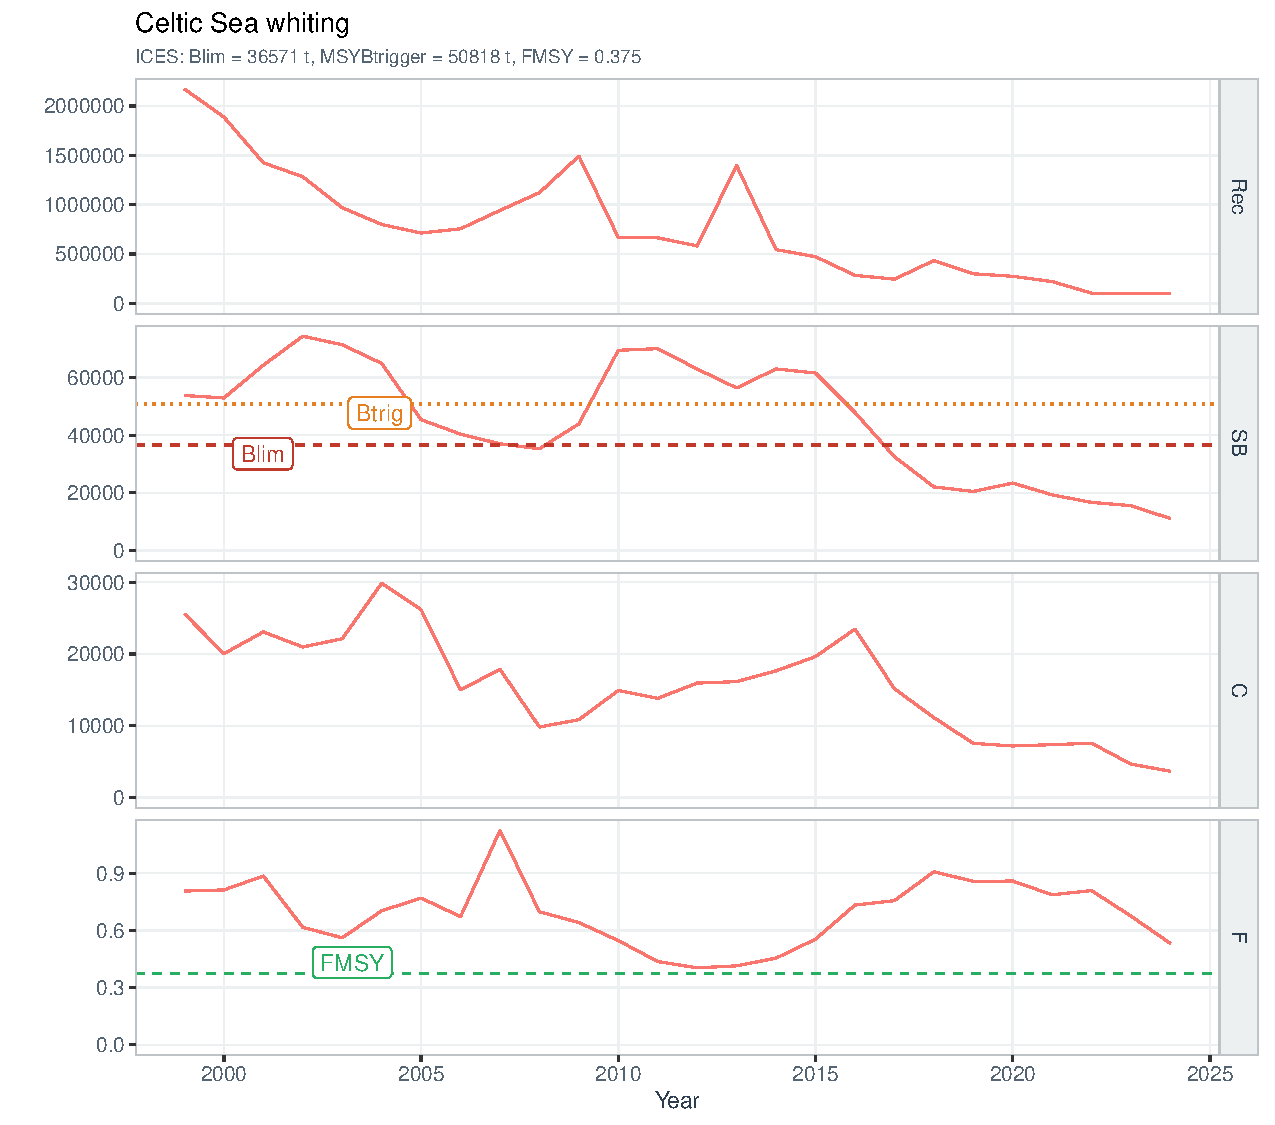
\includegraphics[width=\textwidth]{figs/si/si_flstock_whg.27.7b-ce-k.pdf}
\caption{Celtic Sea whiting (\texttt{whg.27.7b-ce-k}). WGCSE assessment
recruitment, SSB, catch, and $\bar F$, with ICES $\Blim=36571$\,t,
$\Btrig=50818$\,t, and $\Ftar=0.375$.}
\label{fig:si-whg7bcek}
\end{figure}

\begin{figure}[htbp]
\centering
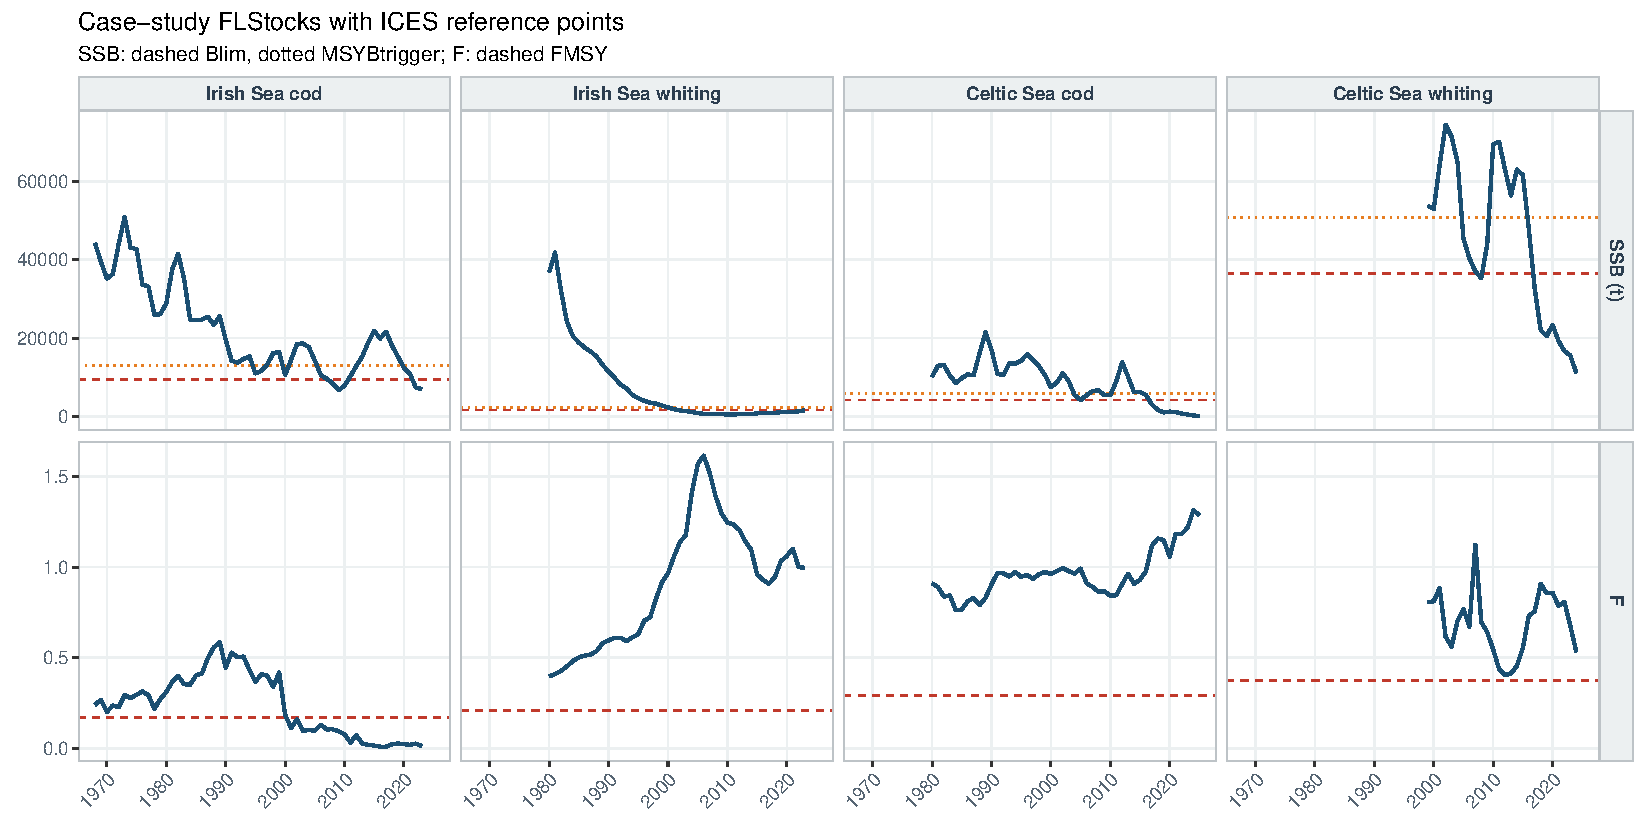
\includegraphics[width=\textwidth]{figs/si/si_flstock_casestudy_overview.pdf}
\caption{Compact overview of the four demonstration stocks: SSB with
$\Blim$ (dashed) and $\Btrig$ (dotted), and $\bar F$ with $\Ftar$
(dashed). Facets use independent $y$-axes.}
\label{fig:si-overview}
\end{figure}

%==============================================================================
\section{Backtest trajectories: Historical, open-loop $\Fmsy$, and Advice rule}
\label{sec:si-backtest-arms}
%==============================================================================

Three trajectories on the conditioned reference OM (Beverton--Holt
stock--recruitment; ICES control points from SAG), shown for the backtest
window only---from the closed-loop start year 2015 through each stock's
terminal assessment year. The policy contrast is Advice rule versus
Historical; open-loop $\Fmsy$ is a no-feedback benchmark only. Future
rebuild projections are omitted here.

\begin{itemize}
  \item \textbf{Historical} --- realised WGCSE assessment path
        (assessment $F$, SSB, recruitment, catch).
  \item \textbf{Open-loop $\Fmsy$} --- open-loop projection at the
        published ICES $F_{\mathrm{MSY}}$ (equal to $\Ftar$ in the advice
        rule); not a second HCR policy. The series is produced from about
        1990 but is plotted only over 2015 to the terminal year.
  \item \textbf{Advice rule} --- closed-loop ICES Category~1 hockey-stick
        as coded, from 2015.
\end{itemize}
% Code: 04.1_openLoop.Rmd (openloop_start), 04.2_closedLoop.Rmd (hcrICES),
% 04.3_rebuild.Rmd (Future; omitted here).

Year ranges: Celtic Sea cod 2015--2025; Irish Sea whiting and Irish Sea
cod 2015--2023; Celtic Sea whiting 2015--2024. Horizontal lines are ICES
$\Blim$, $\Btrig$, and $\Ftar$.

\begin{figure}[htbp]
\centering
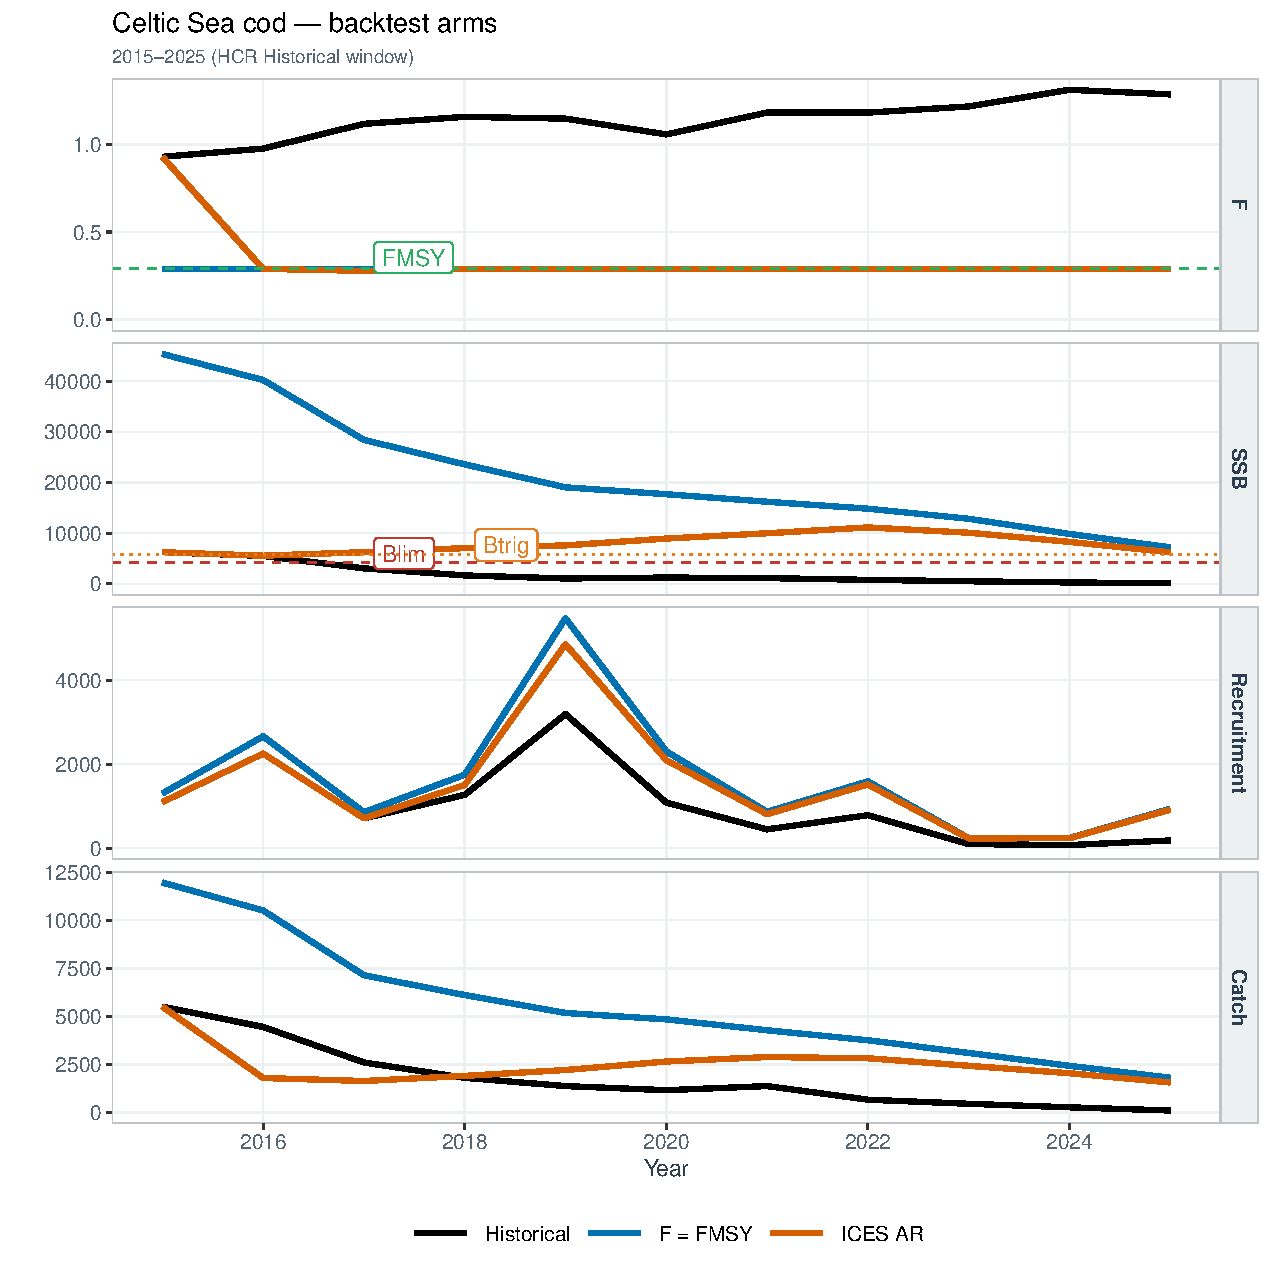
\includegraphics[width=\textwidth]{figs/si/si_backtest_cod.27.7e-k.pdf}
\caption{Celtic Sea cod (\texttt{cod.27.7e-k}): Historical, open-loop
$\Fmsy$ (benchmark), and Advice rule over the backtest window
2015--2025. Panels: $\bar F$, SSB, recruitment, catch.}
\label{fig:si-backtest-cod7ek}
\end{figure}

\begin{figure}[htbp]
\centering
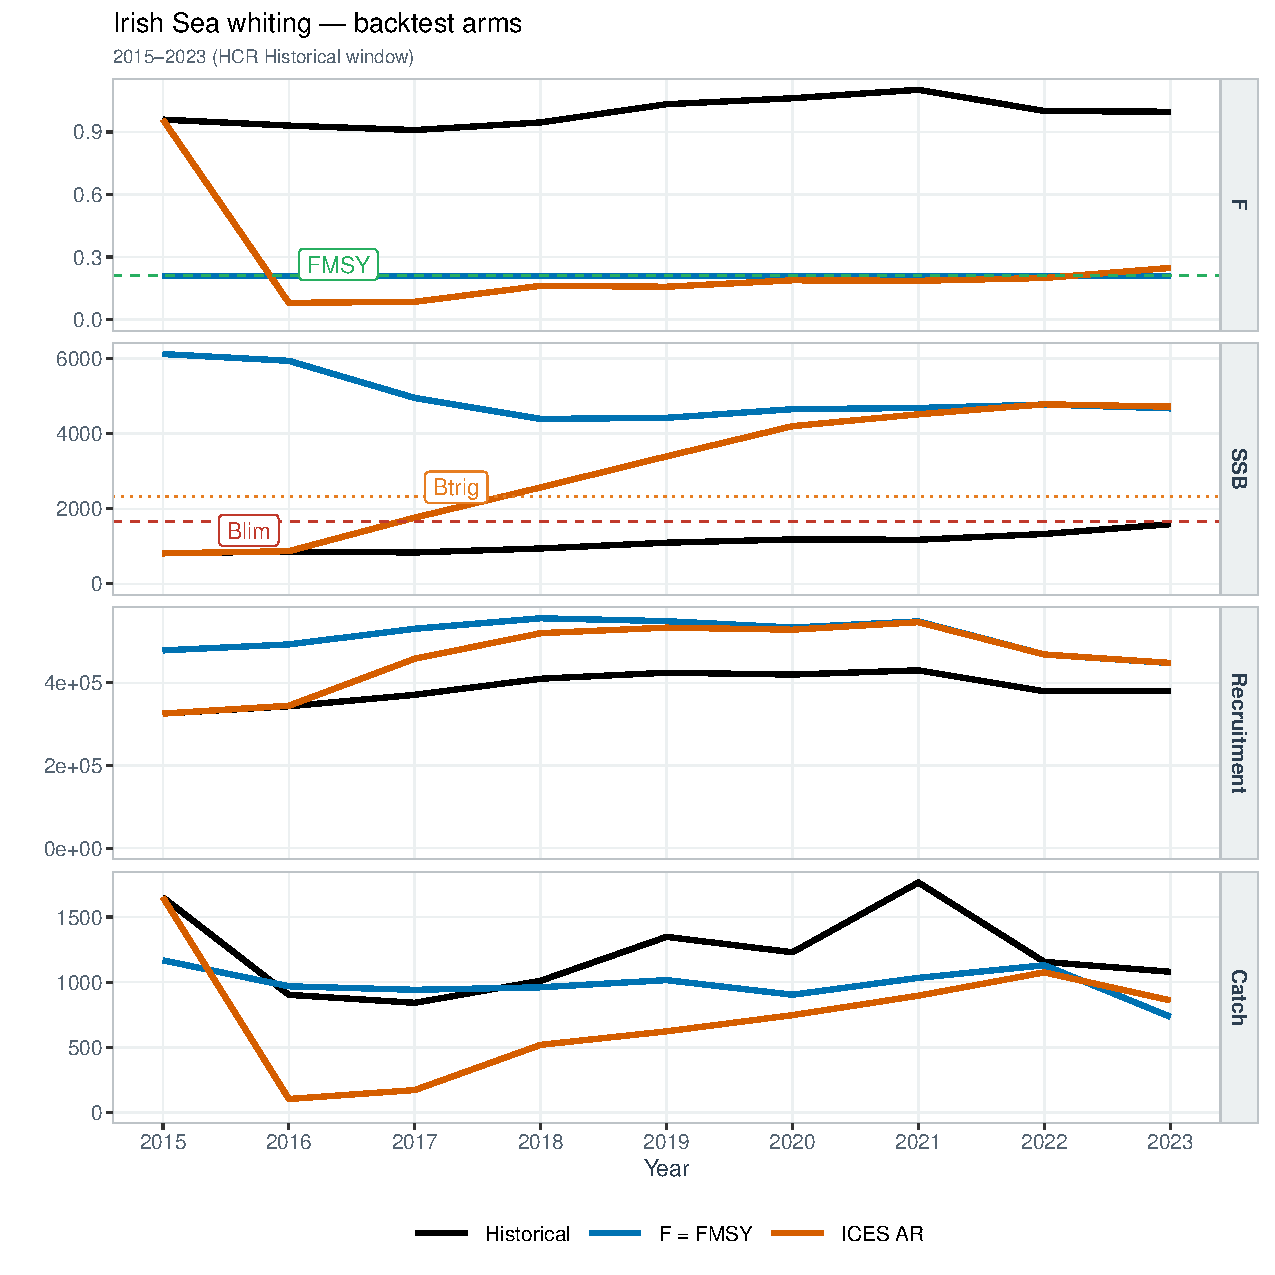
\includegraphics[width=\textwidth]{figs/si/si_backtest_whg.27.7a.pdf}
\caption{Irish Sea whiting (\texttt{whg.27.7a}): Historical, open-loop
$\Fmsy$ (benchmark), and Advice rule over the backtest window
2015--2023.}
\label{fig:si-backtest-whg7a}
\end{figure}

\begin{figure}[htbp]
\centering
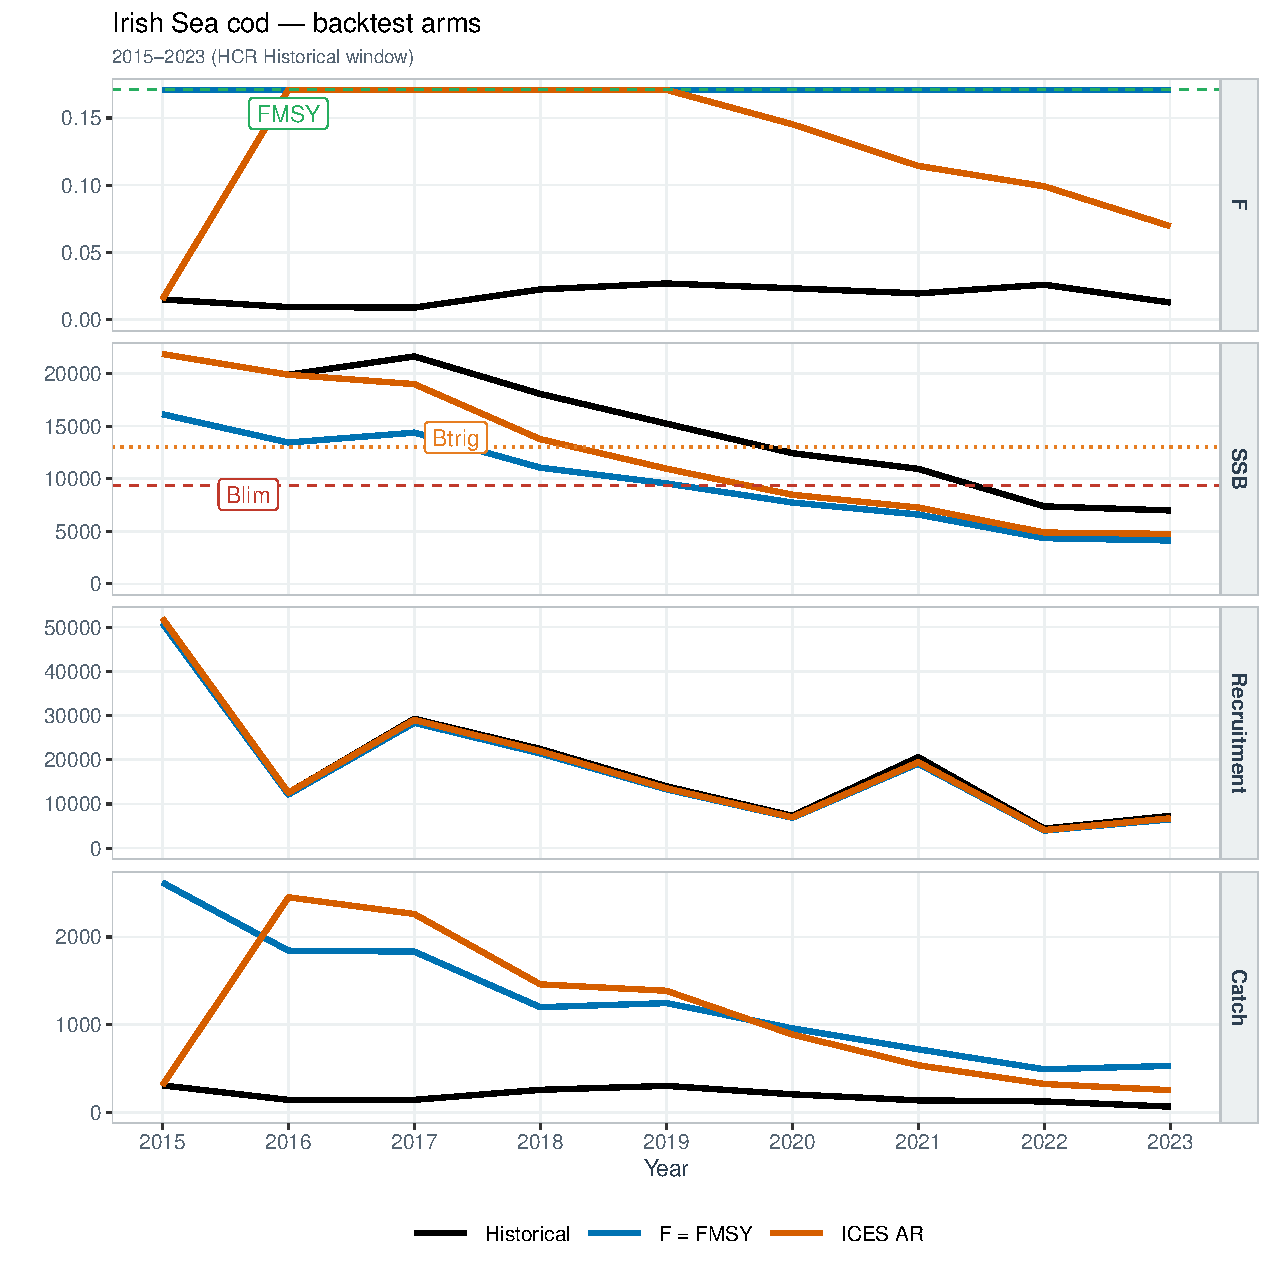
\includegraphics[width=\textwidth]{figs/si/si_backtest_cod.27.7a.pdf}
\caption{Irish Sea cod (\texttt{cod.27.7a}): Historical, open-loop $\Fmsy$
(benchmark), and Advice rule over the backtest window 2015--2023.}
\label{fig:si-backtest-cod7a}
\end{figure}

\begin{figure}[htbp]
\centering
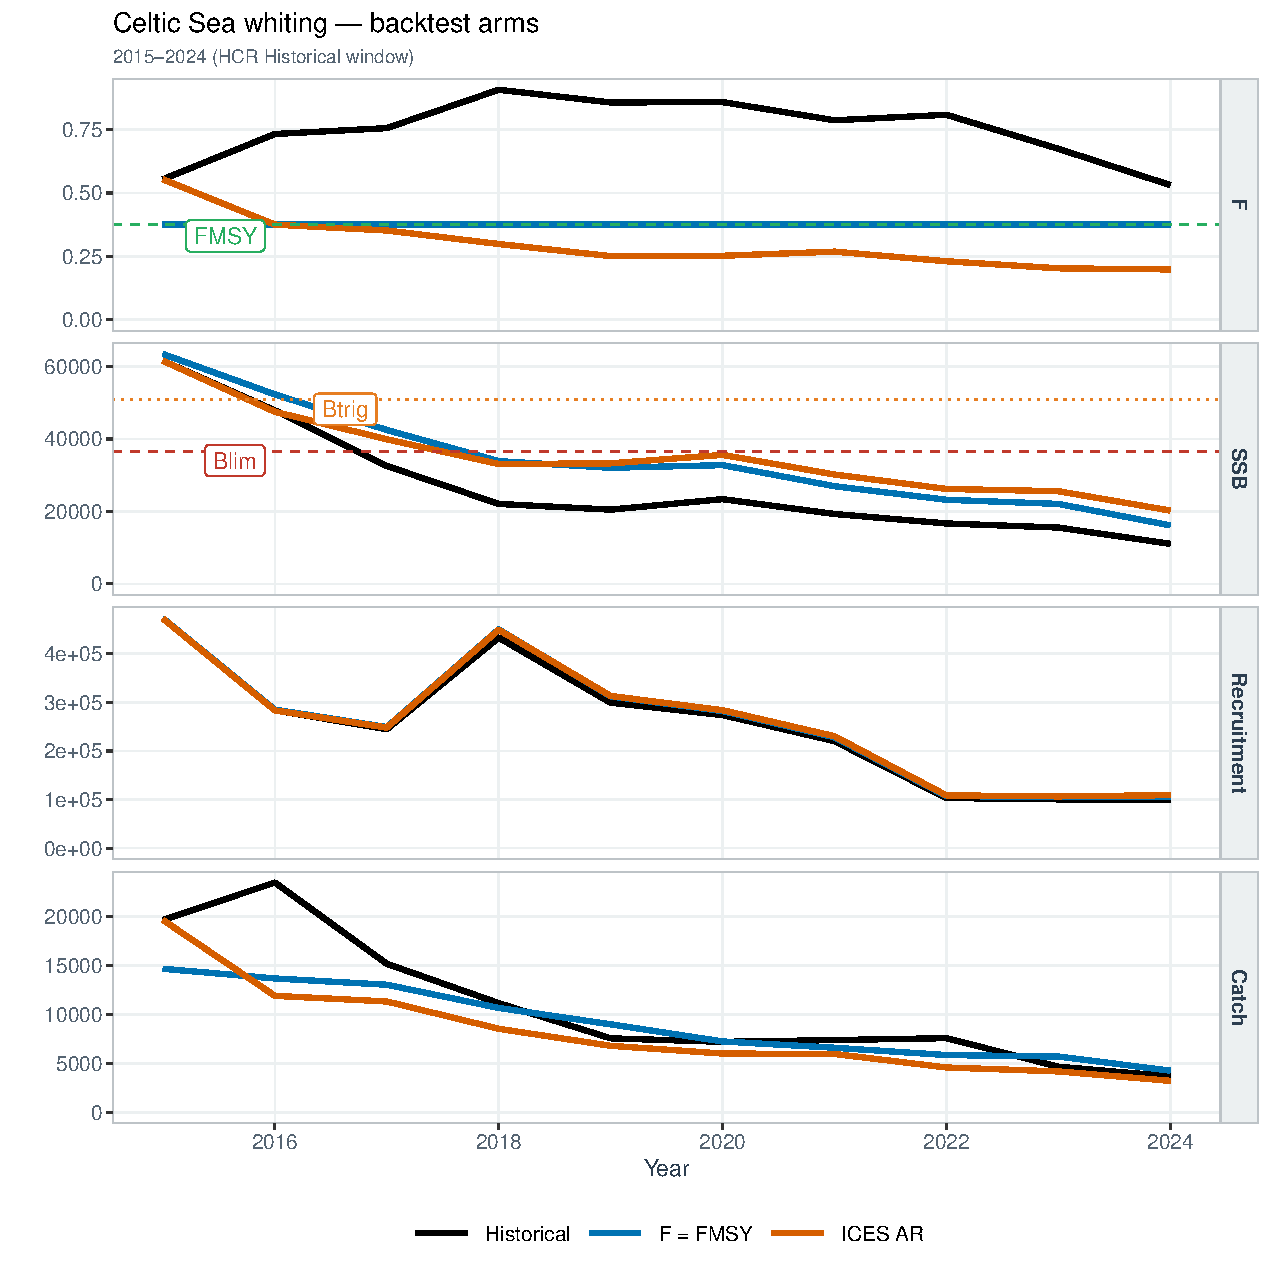
\includegraphics[width=\textwidth]{figs/si/si_backtest_whg.27.7b-ce-k.pdf}
\caption{Celtic Sea whiting (\texttt{whg.27.7b-ce-k}): Historical,
open-loop $\Fmsy$ (benchmark), and Advice rule over the backtest window
2015--2024.}
\label{fig:si-backtest-whg7bcek}
\end{figure}

\begin{figure}[htbp]
\centering
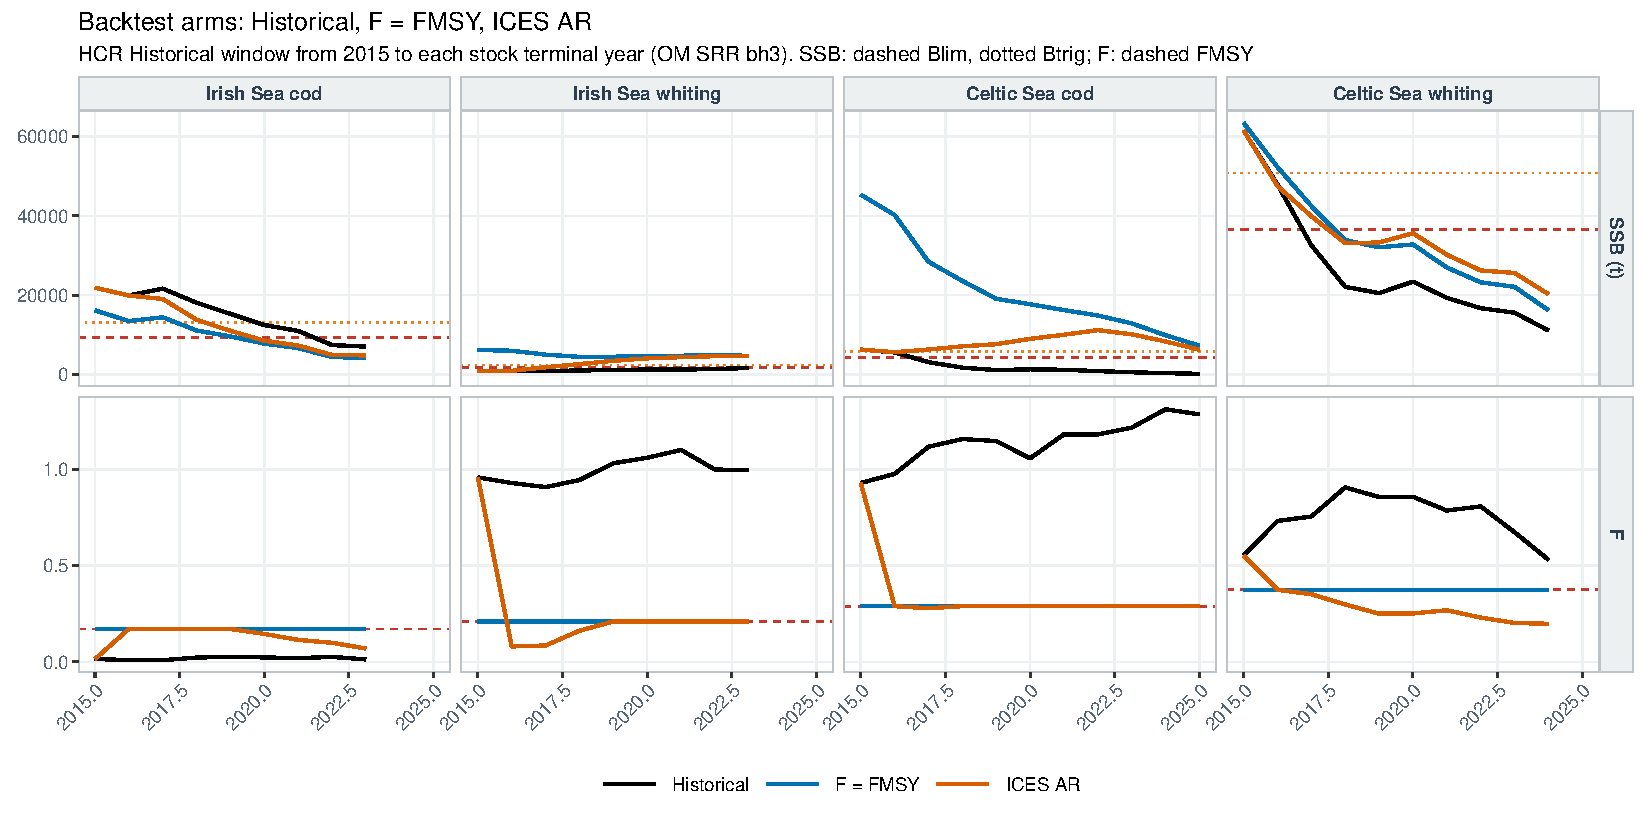
\includegraphics[width=\textwidth]{figs/si/si_backtest_casestudy_overview.pdf}
\caption{Compact overview of Historical, open-loop $\Fmsy$ (benchmark),
and Advice rule for the four demonstration stocks over each stock's
backtest window (2015 to terminal year). SSB with $\Blim$ (dashed) and
$\Btrig$ (dotted); $\bar F$ with $\Ftar$ (dashed). Facets use
independent $y$-axes.}
\label{fig:si-backtest-overview}
\end{figure}

%==============================================================================
\section{Advice versus reported catch}
\label{sec:si-advice-catch}
%==============================================================================

ICES advised catch (Advice and Scenarios Database, ASD) versus reported
catch from the latest SAG assessment year is shown in the advice-versus-
catch figure of the main text. The same four-stock panel is repeated here
for standalone reading of the supplement.

\begin{figure}[htbp]
\centering
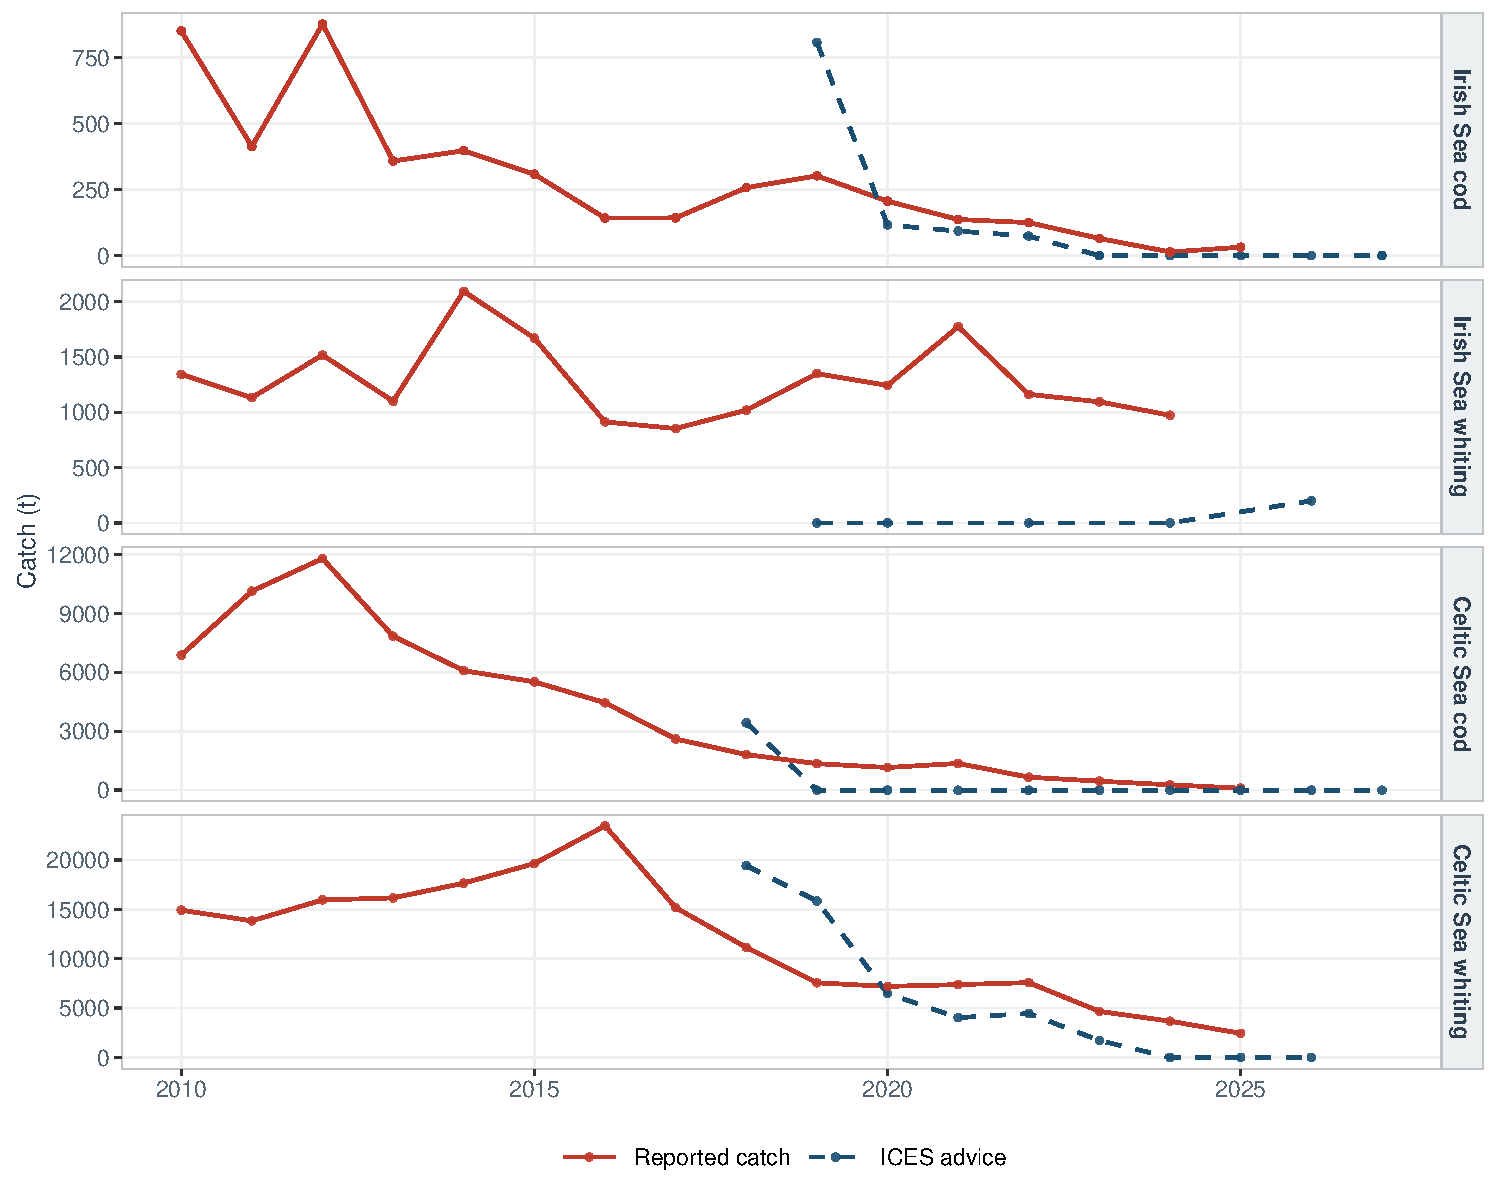
\includegraphics[width=\textwidth]{figs/advice_catch_casestudy.pdf}
\caption{ICES advised catch (ASD) and reported catch (SAG) for the four
demonstration stocks, 2010 onward. Facets use independent $y$-axes
(tonnes).}
\label{fig:si-advice-catch}
\end{figure}
% Source: Rmd/01_screening.Rmd.

% Optional SI additions for a journal version (not part of the funder
% deliverable): OM-gate trajectories (ltermEq / ltermPass) from 02.1/02.2.

\end{document}
